%\documentclass{article}
\documentclass[letter,12pt,oneside]{book}
\usepackage[utf8]{inputenc}
\usepackage[spanish]{babel}
\usepackage[LGR,T1]{fontenc}
\usepackage{amssymb}                % símbolos especiales
\usepackage{amsmath, amsthm}        % ambiente \newtheorem
\usepackage{color}
\usepackage{enumitem}
\usepackage{fancyhdr}
\usepackage{graphicx}
\usepackage{tabto}                  % \tabto
\usepackage{tikz}
\usetikzlibrary{arrows,positioning, calc,automata}
\tikzstyle{vertex}=[draw,fill=black!15,circle,minimum size=20pt,inner sep=0pt]
\setlength{\textheight}{23cm}
\setlength{\textwidth}{18cm}
\setlength{\topmargin}{-1cm}
\setlength{\oddsidemargin}{-1cm}
\setlength{\evensidemargin}{0cm}

% \newtheorem{nombre}{caption}[within]
\theoremstyle{definition}
\newtheorem{corolary}{Corolario}[]
\newtheorem{lemma}{Lema}[]
\newtheorem{theorem}{Teorema}[]
\newtheorem{example}{Ejemplo}[section]

% \newenvironment{nombre}[argumentos]{begindef}{enddef}
\newenvironment{lista}{\begin{list}{\textbullet}{\itemindent -1ex \itemsep -1ex}}{\end{list}}

%-------------------- codigo en Python
% Default fixed font does not support bold face
\DeclareFixedFont{\ttb}{T1}{txtt}{bx}{n}{12} % for bold
\DeclareFixedFont{\ttm}{T1}{txtt}{m}{n}{12}  % for normal

% Custom colors
\usepackage{color}
\definecolor{deepblue}{rgb}{0,0,0.5}
\definecolor{deepred}{rgb}{0.6,0,0}
\definecolor{deepgreen}{rgb}{0,0.5,0}

\usepackage{listings}

\pagenumbering{gobble}

%---------------------------- hasta aqui

\rhead{\begin{picture}(0,0) \put(-120,0){
\includegraphics[width=40mm]{./image/logo-UV}} \end{picture}}
\lhead{\vspace{-0.3cm}Universidad de Valparaíso\\Facultad de Ingeniería\\Escuela de Ingeniería Civil Informática\vspace{0.1cm}}

\pagestyle{fancy}

\begin{document}
%\maketitle

\begin{center}
$~$
\end{center}

\noindent
Nombre: \rule{.6\textwidth}{.5pt} Rut: \rule{.24\textwidth}{.5pt}

\begin{center}
 {\Large
  {\color{white}.}\\
  Estructuras de datos\\[1ex]
  Control 6 (Fila A)}\\[1.2ex]
  Prof: Fabián Riquelme Csori\\
  2017-II
\end{center}

\begin{minipage}[t]{0.57\textwidth}
  \vspace{-3cm}
  
  \begin{enumerate}
    \item Una nueva empresa de telecomunicaciones se quiere instalar en la Región de Valparaíso para proveer de Internet a toda la zona. Para eso deben instalar un número de antenas repetidoras en distintas provincias de la región (representada en el mapa) utilizando la menor cantidad de recursos posibles. La capacidad tecnológica de la empresa permite que si una antena se instala en una provincia, esta alcance a proveer de señal tanto a dicha provincia como a sus provincias vecinas.
    \begin{enumerate}
        \item Modele el sistema como un grafo, explicando qué representan los vértices y qué representan las aristas. \tabto{38ex} [10 pts]
    \end{enumerate}
  \end{enumerate}
\end{minipage}
\begin{minipage}[h]{0.4\textwidth}
    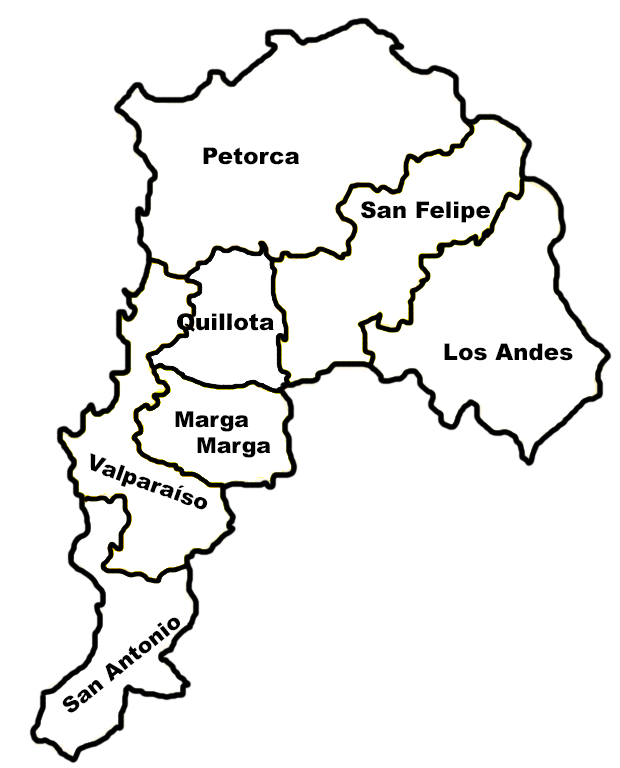
\includegraphics[width=\textwidth]{./image/cap6/mapa-valpo.png}
\end{minipage}
  \begin{enumerate}
      {\setlength\itemindent{43pt} \item[b)] ¿Qué problema de grafos visto en clase calza mejor con este? Fundamente. \tabto{86ex} [10 pts]}
  \end{enumerate}
  \begin{enumerate}
    \item[2.] En el Aula Virtual hay un archivo llamado \texttt{grafo-control6-filaA.csv}, donde \texttt{A} es la fila correspondiente a su Control. Dicho archivo contiene un grafo representado como una lista de aristas.
    \begin{enumerate}
        \item ¿Cuál es el orden y el número de aristas del grafo? \tabto{81ex} [10 pts]
        \item ¿Se trata de un grafo denso o disperso? Fundamente. \tabto{81ex} [15 pts]
        \item ¿Cuál es el camino más corto para llegar del vértice 1 hasta el vértice 10?\\[1.5ex]
        \textbf{Tip:} Para resolver este problema puede implementar un pequeño programa reutilizando código desarrollado en clases. No se pide el código, solo su respuesta y argumentos, en base a los resultados obtenidos. No se pide eficiencia. \tabto{81ex} [15 pts]
    \end{enumerate}
\end{enumerate}

\newpage
\noindent
Nombre: \rule{.6\textwidth}{.5pt} Rut: \rule{.24\textwidth}{.5pt}

\begin{center}
 {\Large
  {\color{white}.}\\
  Estructuras de datos\\[1ex]
  Control 6 (Fila B)}\\[1.2ex]
  Prof: Fabián Riquelme Csori\\
  2017-II
\end{center}

\begin{minipage}[t]{0.57\textwidth}
  \vspace{-3cm}
  
  \begin{enumerate}
    \item Una nueva empresa de telecomunicaciones se quiere instalar en la Región de Valparaíso para proveer de Internet a toda la zona. Para eso deben instalar un número de antenas repetidoras en distintas provincias de la región (representada en el mapa) utilizando la menor cantidad de recursos posibles. La capacidad tecnológica de la empresa permite que si una antena se instala en una provincia, esta alcance a proveer de señal tanto a dicha provincia como a sus provincias vecinas.
    \begin{enumerate}
        \item Modele el sistema como un grafo, explicando qué representan los vértices y qué representan las aristas. \tabto{38ex} [10 pts]
    \end{enumerate}
  \end{enumerate}
\end{minipage}
\begin{minipage}[h]{0.4\textwidth}
    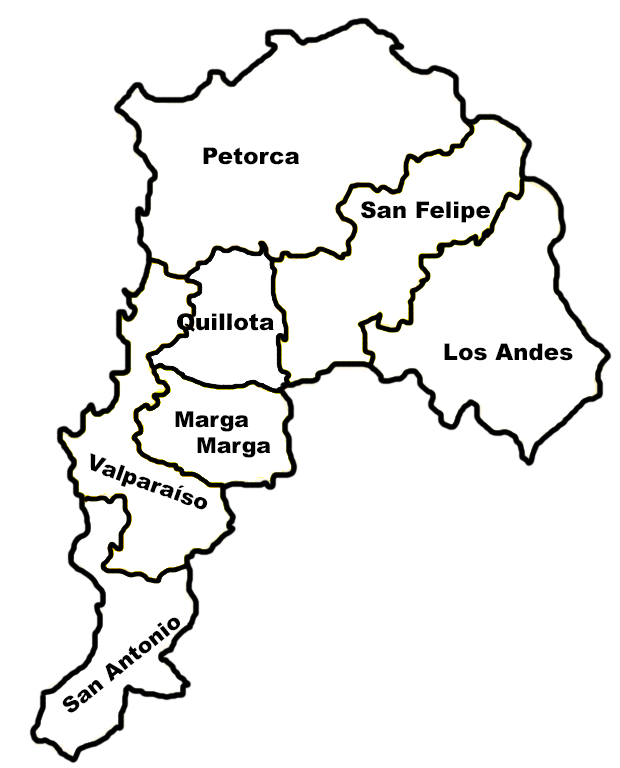
\includegraphics[width=\textwidth]{./image/cap6/mapa-valpo.png}
\end{minipage}
  \begin{enumerate}
      {\setlength\itemindent{43pt} \item[b)] ¿Qué problema de grafos visto en clase calza mejor con este? Fundamente. \tabto{86ex} [10 pts]}
  \end{enumerate}
  \begin{enumerate}
    \item[2.] En el Aula Virtual hay un archivo llamado \texttt{grafo-control6-filaB.csv}, donde \texttt{B} es la fila correspondiente a su Control. Dicho archivo contiene un grafo representado como una lista de aristas.
    \begin{enumerate}
        \item ¿Cuál es el orden y el número de aristas del grafo? \tabto{81ex} [10 pts]
        \item ¿Se trata de un grafo denso o disperso? Fundamente. \tabto{81ex} [15 pts]
        \item ¿Cuál es el camino más corto para llegar del vértice 1 hasta el vértice 10?\\[1.5ex]
        \textbf{Tip:} Para resolver este problema puede implementar un pequeño programa reutilizando código desarrollado en clases. No se pide el código, solo su respuesta y argumentos, en base a los resultados obtenidos. No se pide eficiencia. \tabto{81ex} [15 pts]
    \end{enumerate}
\end{enumerate}

\newpage
\noindent
Nombre: \rule{.6\textwidth}{.5pt} Rut: \rule{.24\textwidth}{.5pt}

\begin{center}
 {\Large
  {\color{white}.}\\
  Estructuras de datos\\[1ex]
  Control 6 (Pauta)}\\[1.2ex]
  Prof: Fabián Riquelme Csori\\
  2017-II
\end{center}

\begin{enumerate}
    \item[1.a)] El sistema puede modelarse como un grafo $G=(V,E)$ donde: el conjunto de vértices $V=\{SA,V,M,P,Q,SF,LA\}$ representa respectivamente las provincias de San Antonio, Valparaíso, Marga-Marga, Petorca Quillota, San Felipe y Los Andes; \tabto{87ex} [2 pts]\\
    el conjunto de aristas $E$ viene dado por la relación ``limita con'', de modo que una arista $(a,b)\in E$ representa el hecho que las provincias $a$ y $b$ son colindantes. \tabto{87ex} [3 pts]
\begin{center}
\begin{tikzpicture}[-,auto,node distance=2.5cm]
  \tikzstyle{every state}=[draw]

  \node[state] (P)               {$P$};
  \node[state] (SF) [right of=P] {$SF$};
  \node[state] (V)  [below left of=P] {$V$};
  \node[state] (Q)  [below left of=SF] {$Q$};
  \node[state] (LA) [right of=SF] {$LA$};
  \node[state] (SA) [below left of=V] {$SA$};
  \node[state] (MM) [below right of=V] {$M$};
  
  \path (P)  edge node{} (SF)
             edge node{} (V)
             edge node{} (Q)
        (SF) edge node{} (LA)
             edge node{} (Q)
        (V)  edge node{} (Q)
             edge node{} (SA)
             edge node{} (MM)
        (MM) edge node{} (Q)
        ;
\end{tikzpicture}
\end{center}
\tabto{87ex} [5 pts]

    \item[1.b)] El problema de cobertura \tabto{87ex} [5 pts]\\
    de vértices, pues una cobertura de vértices mínima representaría un conjunto de provincias en las cuales ubicar una antena repetidora de modo de proveer de señal a toda la región.\tabto{87ex} [5 pts]\\
    (-5 pts si no hay fundamentación).
    
    \item[2.a)] El orden o número de vértices es 10. \tabto{87ex} [5 pts]\\
    El número de aristas es 20 (una por cada fila, salvo la fila inicial).\tabto{87ex} [5 pts]

    \item[2.b)] Es un grafo disperso, \tabto{87ex} [5 pts]\\
    pues su número de aristas (20) es muchísimo menor al número que podría tener un grafo completo de 10 vértices (90). Análogamente, se podría justificar empleando la fórmula de densidad de un grafo.\tabto{86ex} [10 pts]

    \item[2.c)] Fila A: 1-7-4-5-10 (peso 34)\\
    Fila B: 1-3-4-5-10 (peso 38)\tabto{86ex} [15 pts]\\
    Si la solución no es correcta, hay 5 pts por representar una solución en los términos correctos, como camino de vértices.\\
    A quienes entendieron ``camino más corto'' en el sentido topológico y no de acuerdo con los pesos de las aristas, solo les desconté 5 pts (la ``eficiencia'' se refiere a la ejecución del algoritmo).

\end{enumerate}

\end{document}
